\documentclass[12pt]{article}


\author{Fl\'{a}vio Cruz and Richard Veras}
\title{Assignment 2}

\usepackage{amsmath}
\usepackage{amsfonts}   % if you want the fonts
\usepackage{amssymb}    % if you want extra symbols
%\usepackage{savetrees}
\usepackage{algorithmic}
\usepackage{graphicx}
\usepackage{listings}


\begin{document}
\maketitle

\section{Questions}
\subsection{Lazy Code Motion}

\textbf{Item 1}

\begin{figure}[!htbp]
    \centering
    \caption{CFG after pass 1: anticipated expressions.}
    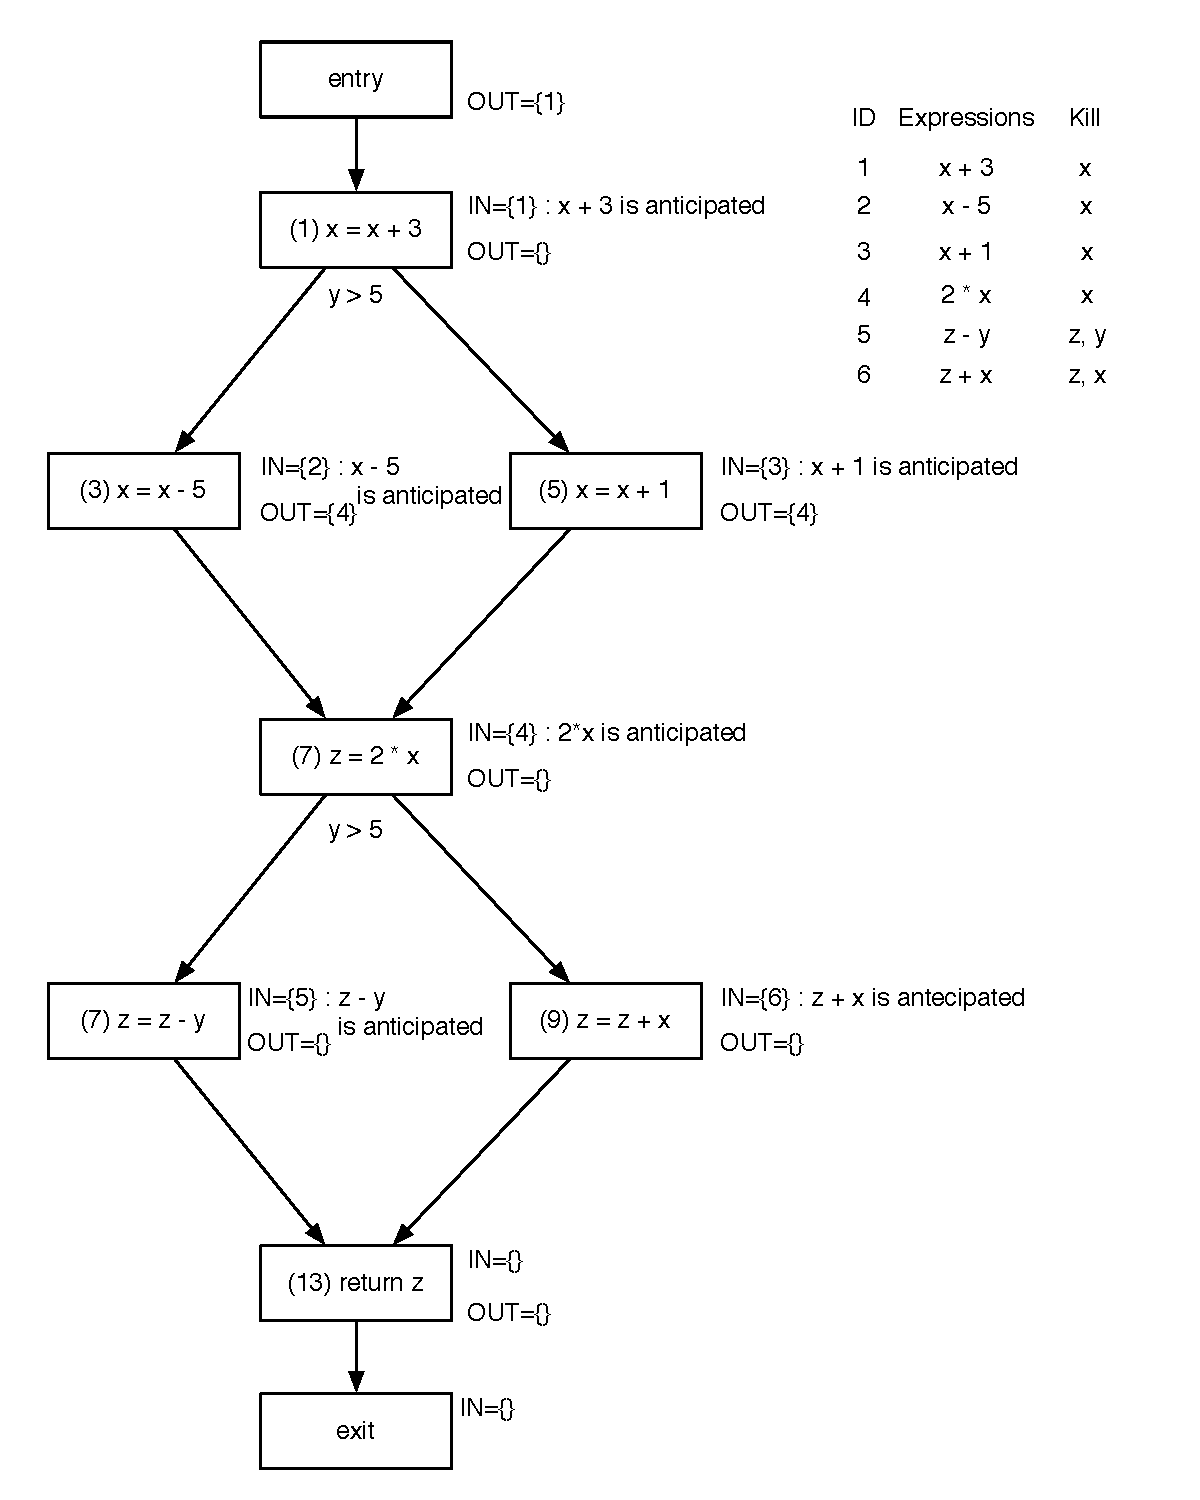
\includegraphics[scale=0.65]{cfg.pdf}
    \label{fig:cfg1}
\end{figure}

\pagebreak

\textbf{Item 2}

\begin{figure}[!htbp]
    \centering
    \caption{CFG after pass 2: early placement.}
    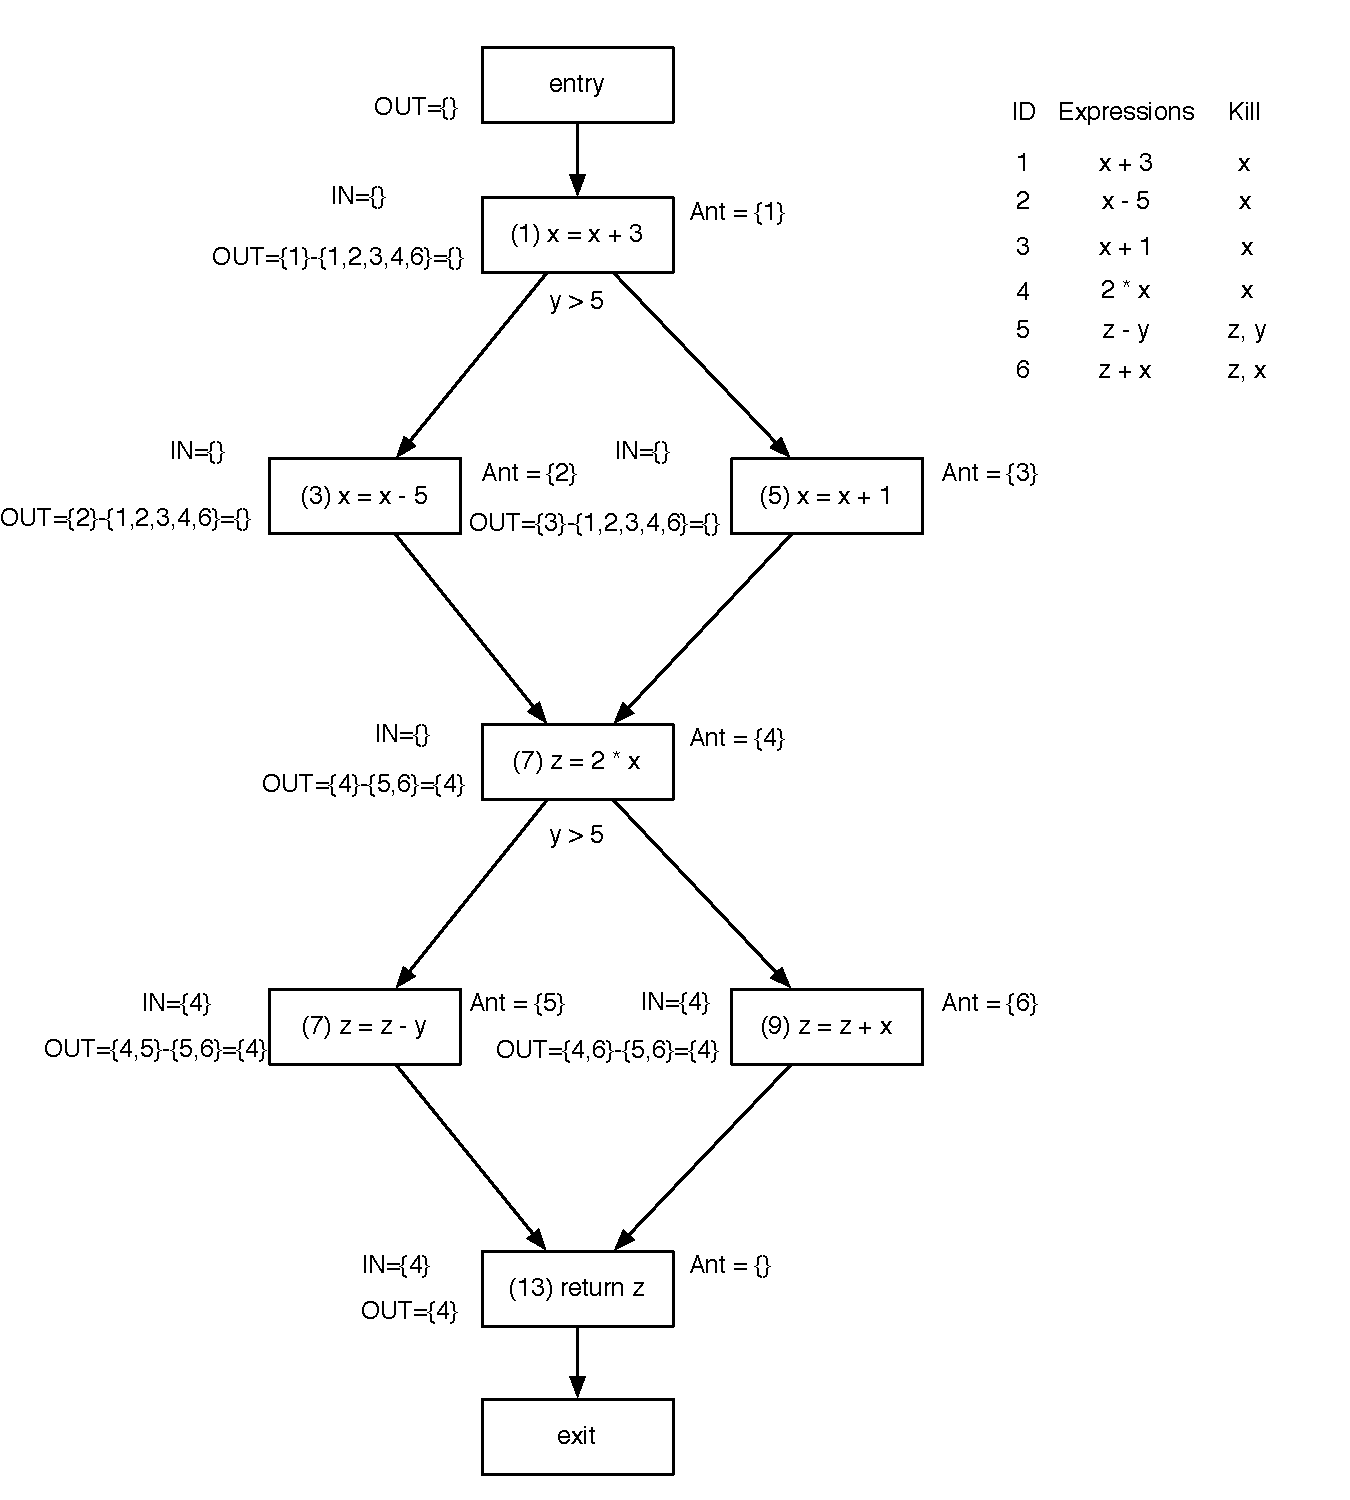
\includegraphics[scale=0.65]{cfg2.pdf}
    \label{fig:cfg2}
\end{figure}

\begin{figure}[!htbp]
    \centering
    \caption{CFG after pass 2: computing \texttt{earliest} and adding instructions.}
    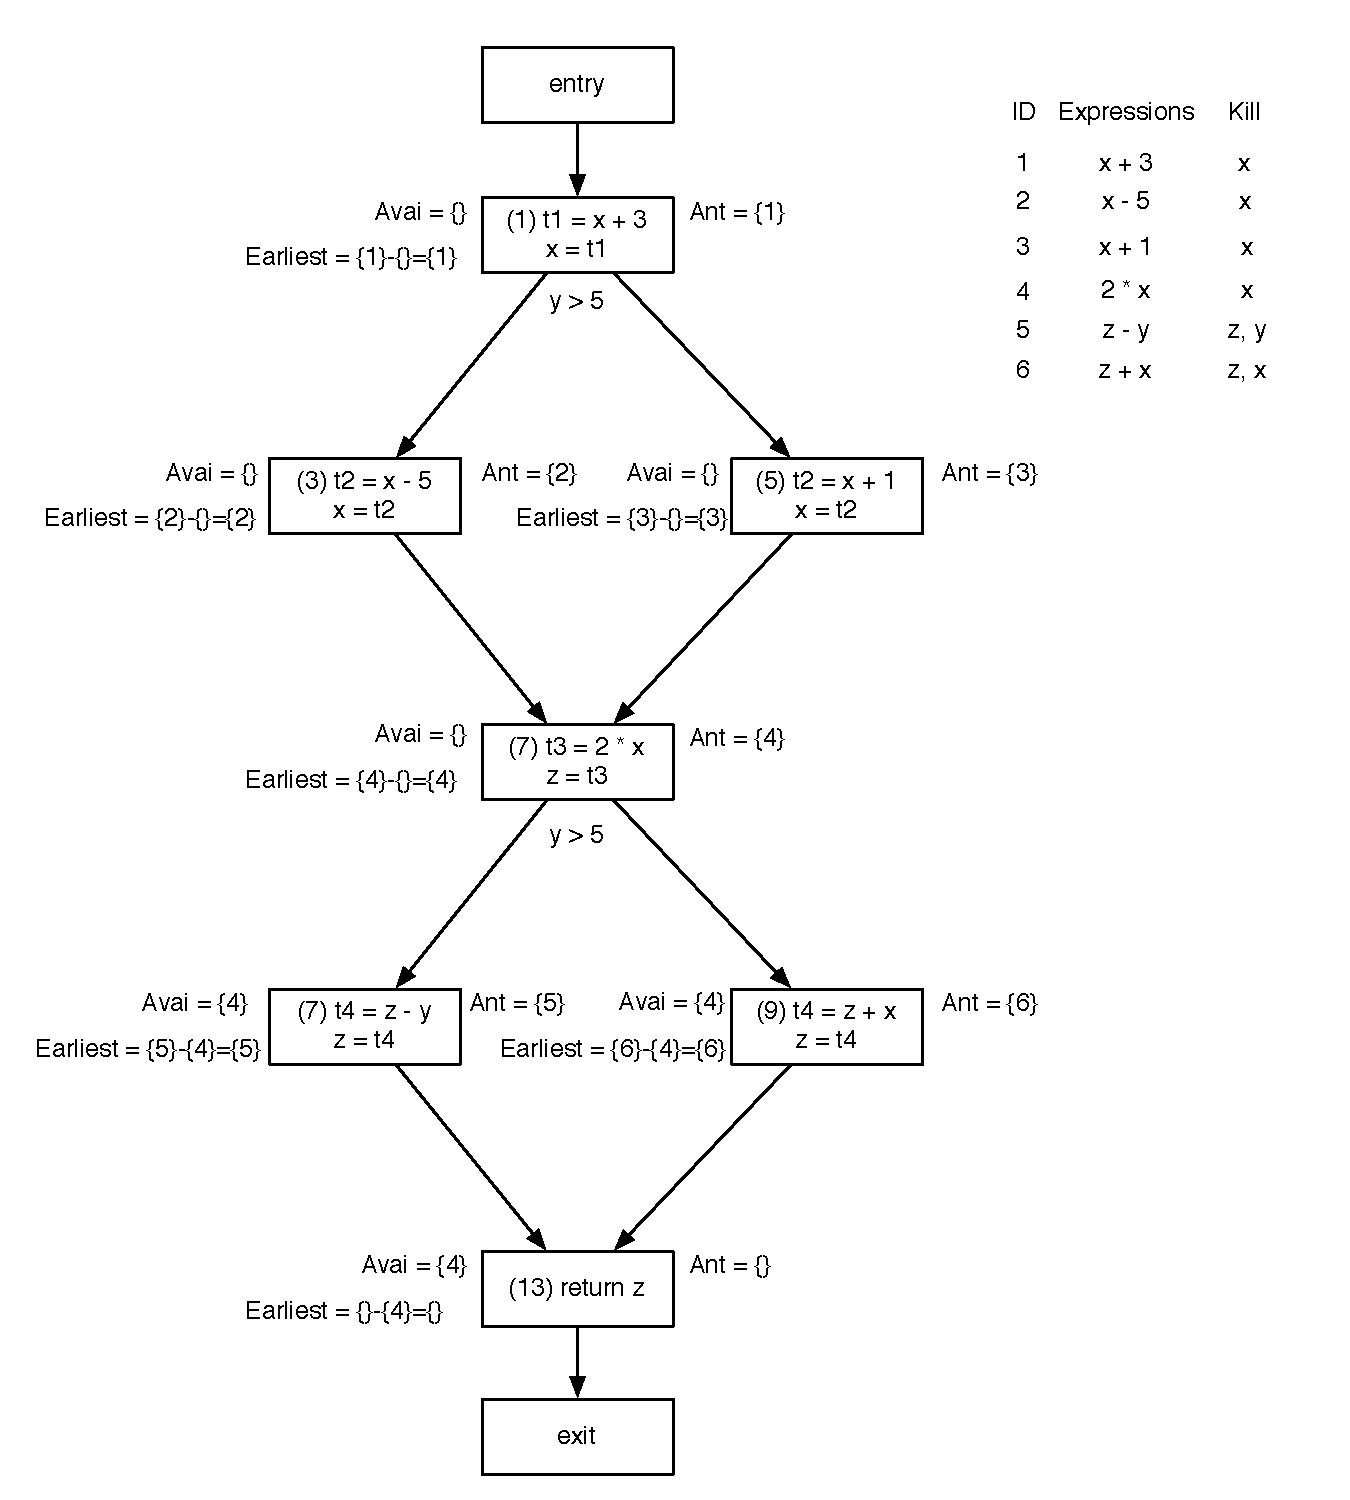
\includegraphics[scale=0.65]{cfg2_1.pdf}
    \label{fig:cfg21}
\end{figure}

\begin{figure}[!htbp]
    \centering
    \caption{CFG after pass 2: constant folding.}
    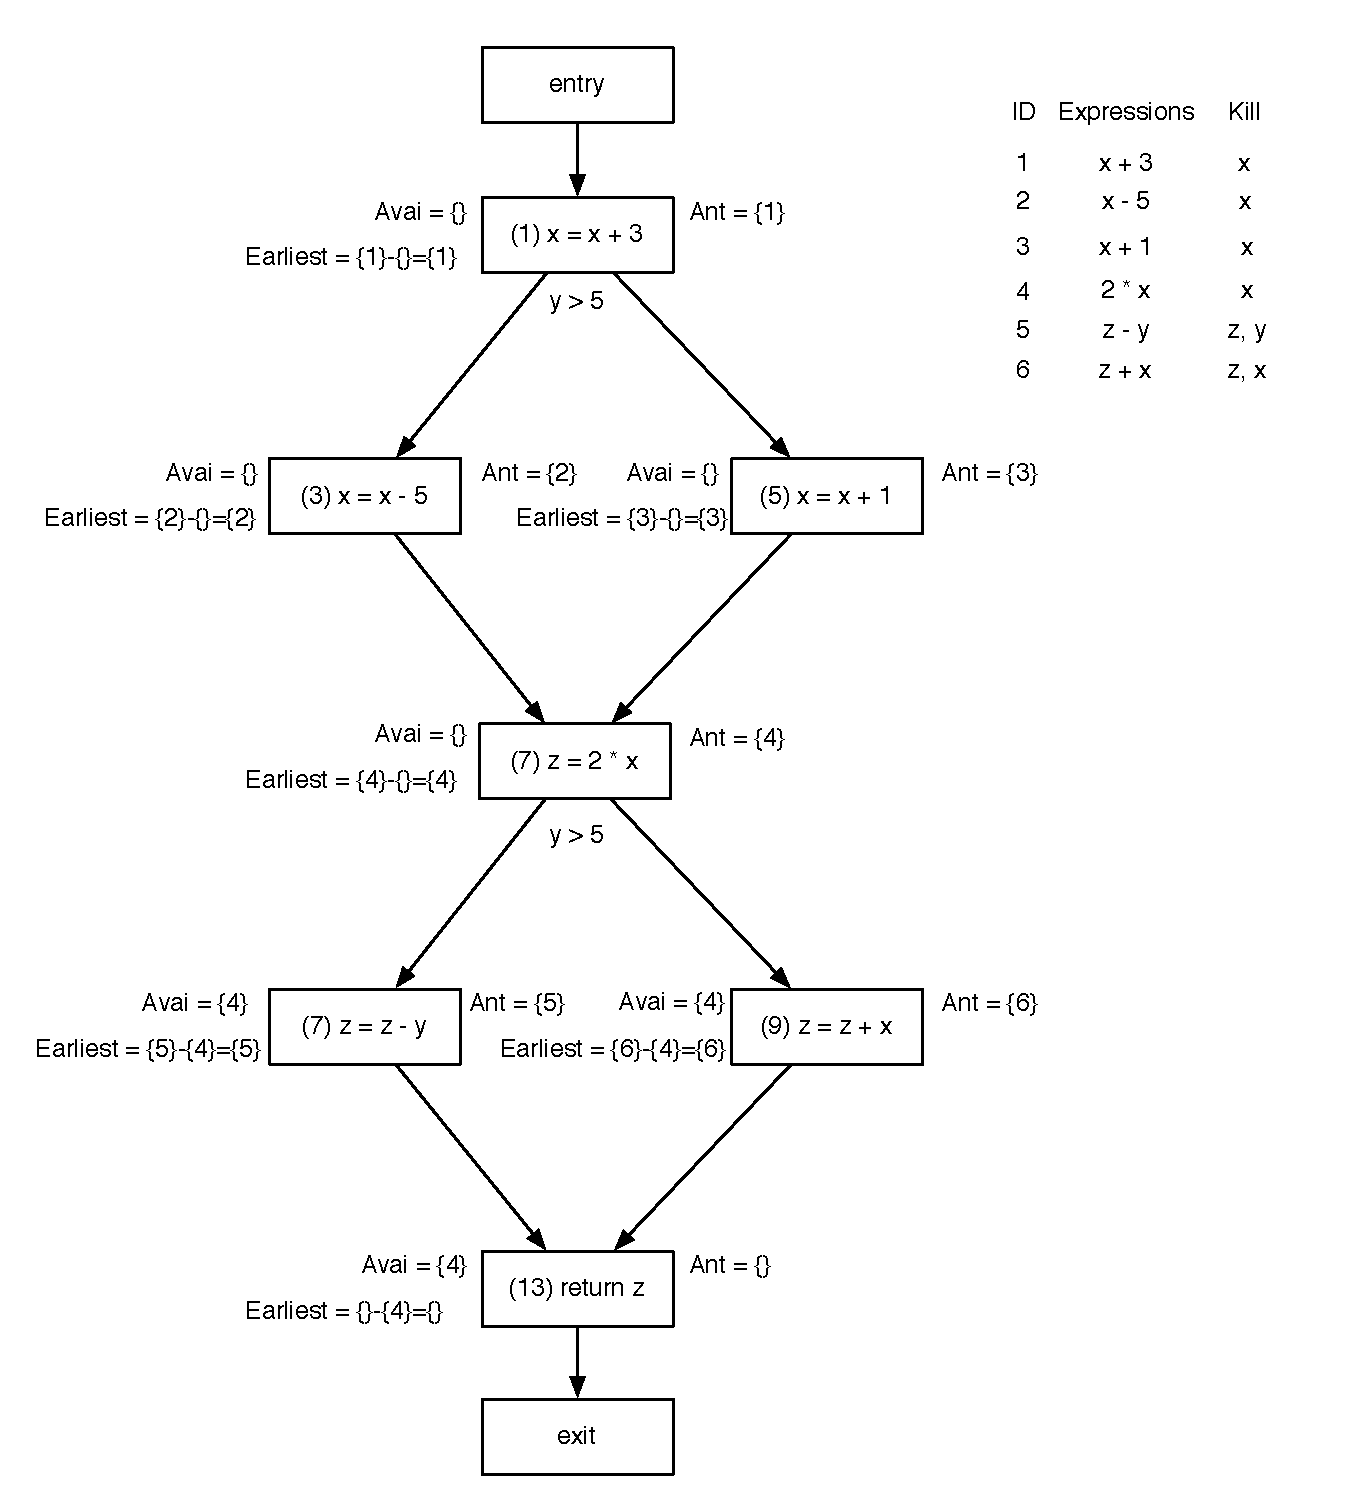
\includegraphics[scale=0.65]{cfg2_2.pdf}
    \label{fig:cfg22}
\end{figure}

\pagebreak

\textbf{Item 3}

\begin{figure}[!htbp]
    \centering
    \caption{CFG after pass 2: cleanup.}
    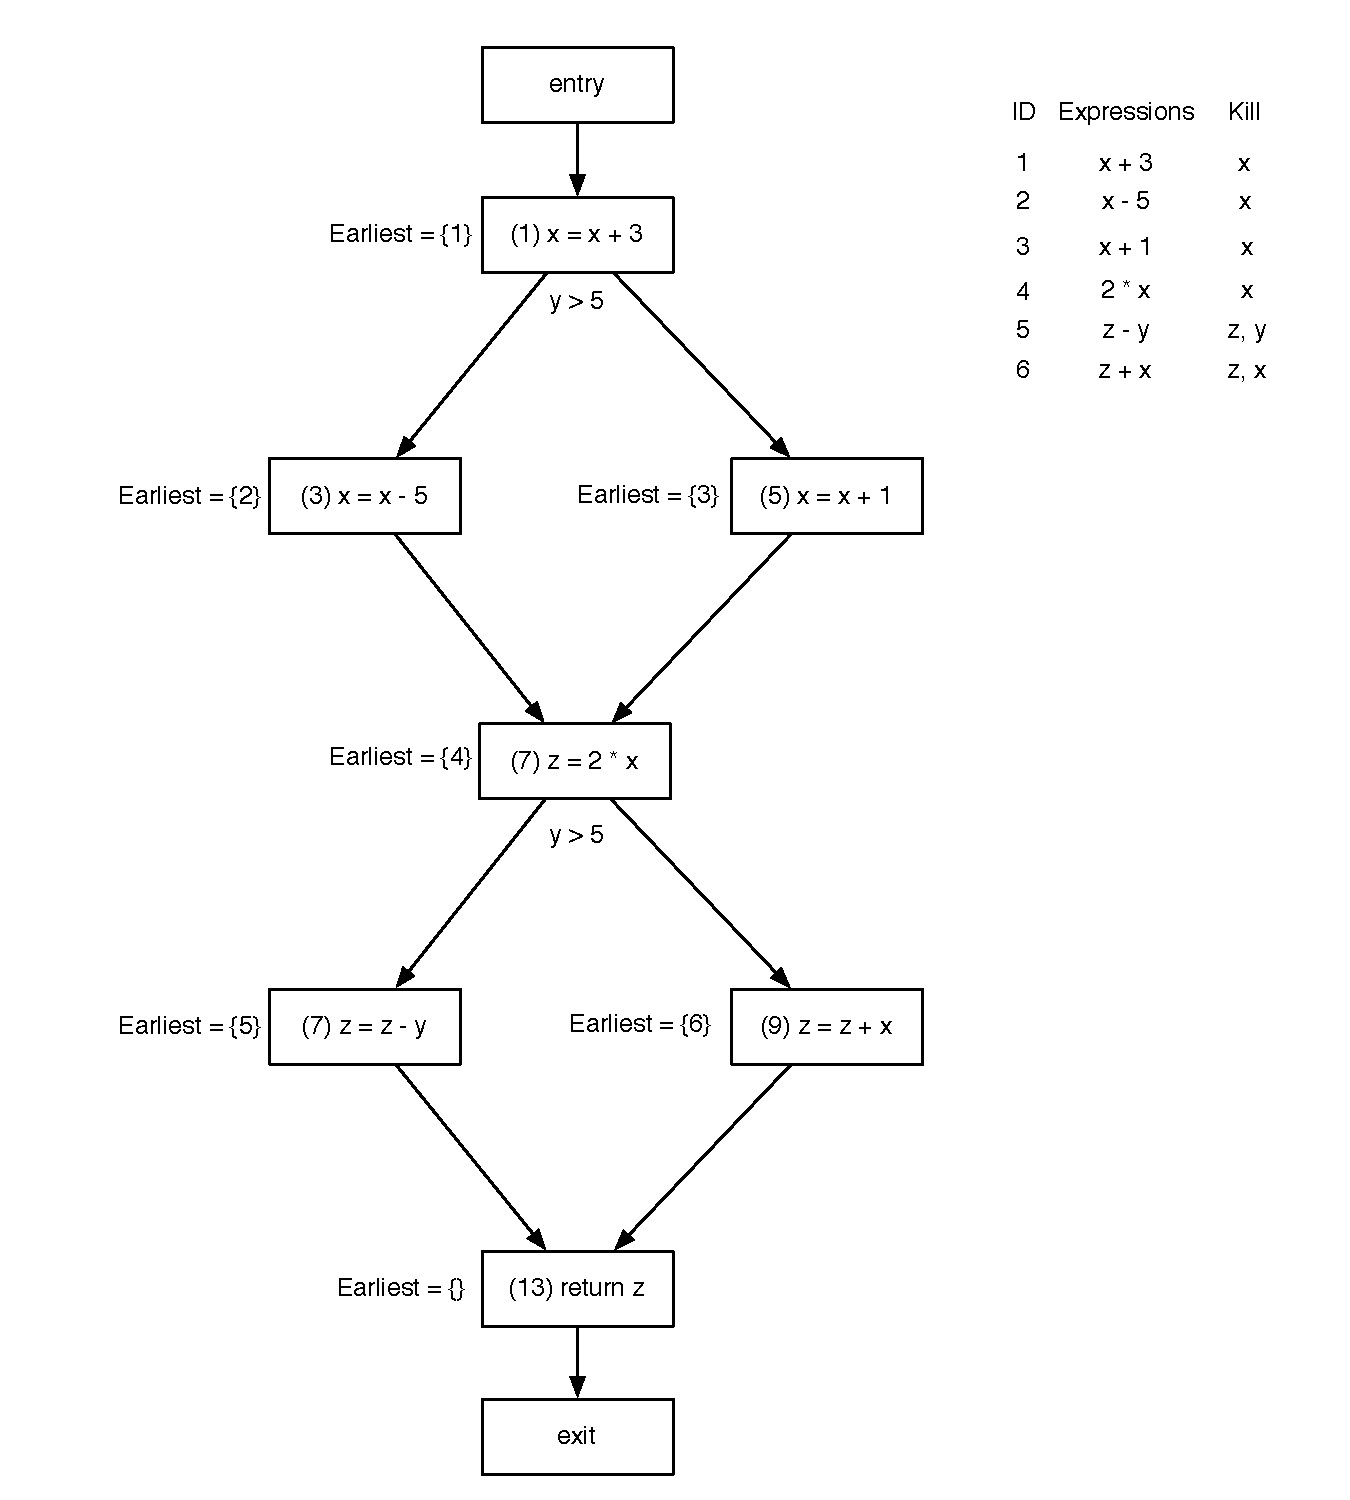
\includegraphics[scale=0.65]{cfg3.pdf}
    \label{fig:cfg3}
\end{figure}

\begin{figure}[!htbp]
    \centering
    \caption{CFG after pass 3: lazy code motion.}
    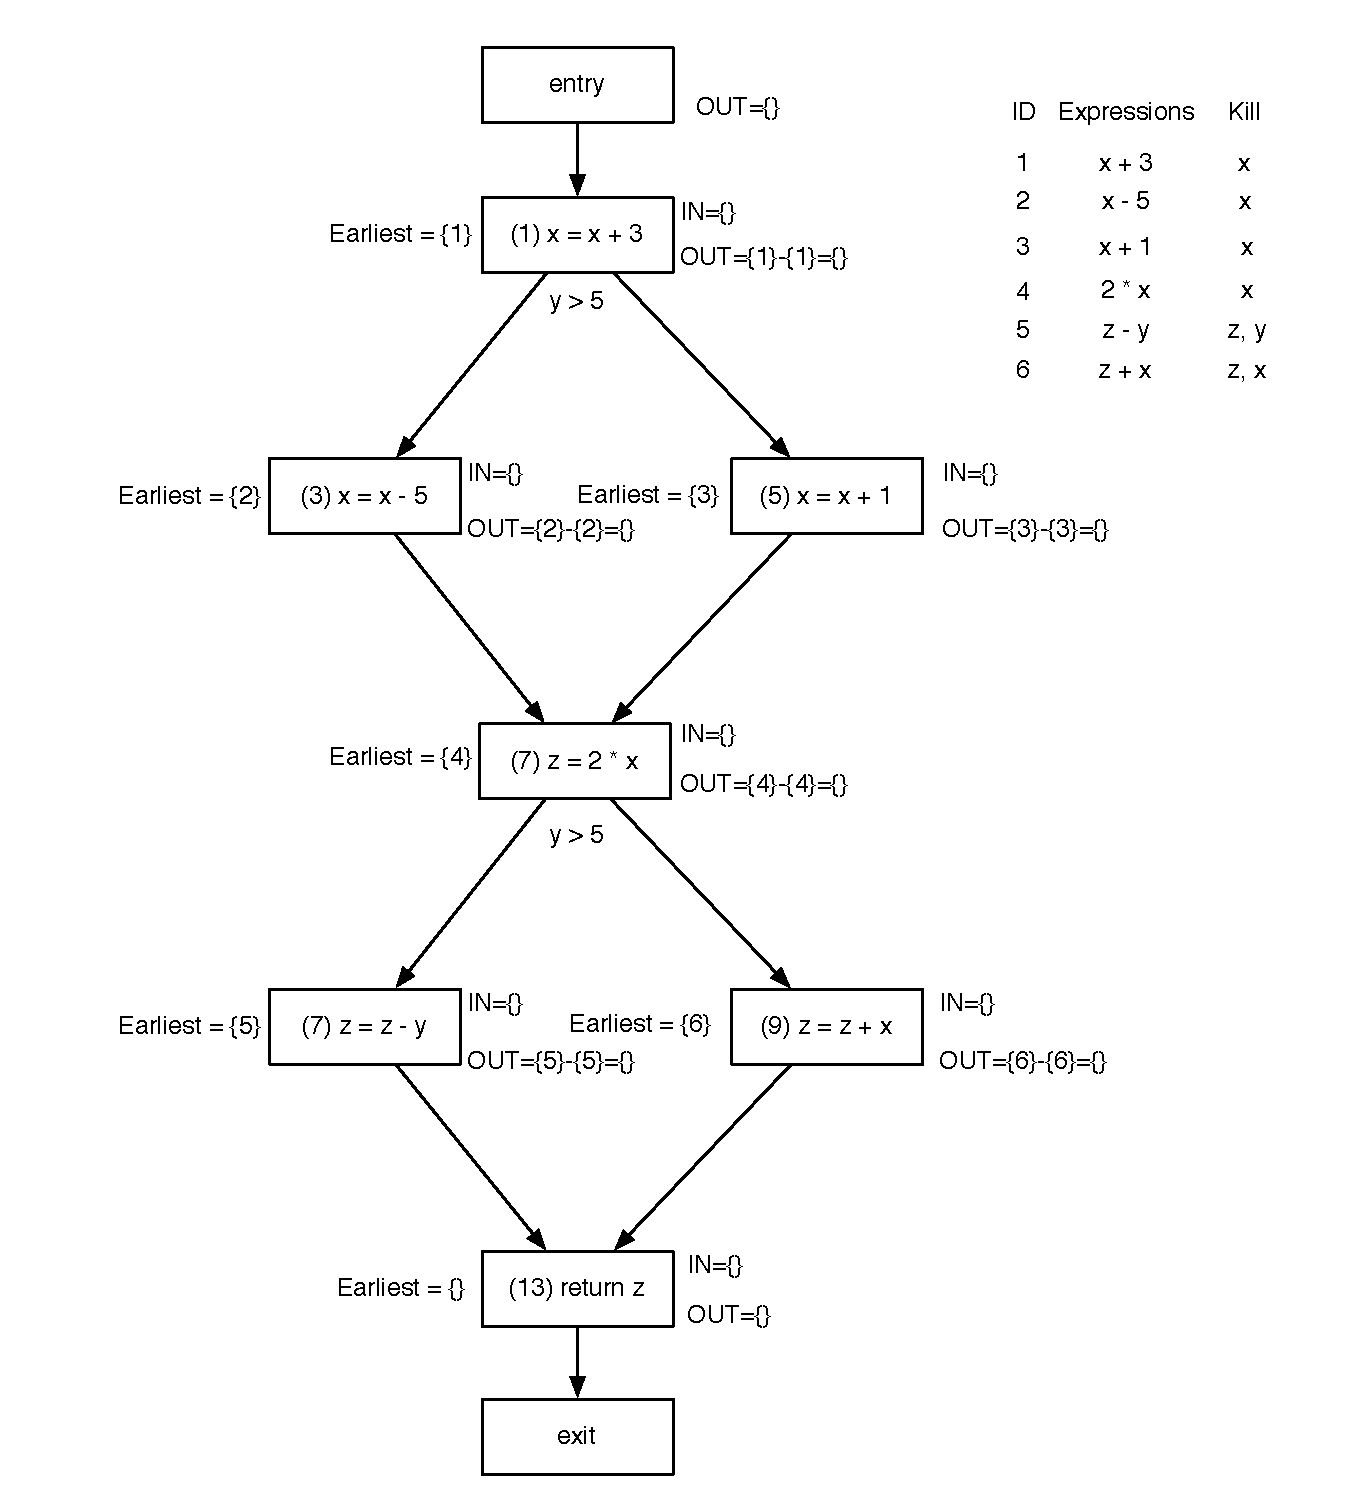
\includegraphics[scale=0.65]{cfg4.pdf}
    \label{fig:cfg4}
\end{figure}

\begin{figure}[!htbp]
    \centering
    \caption{CFG after pass 3: computing latest.}
    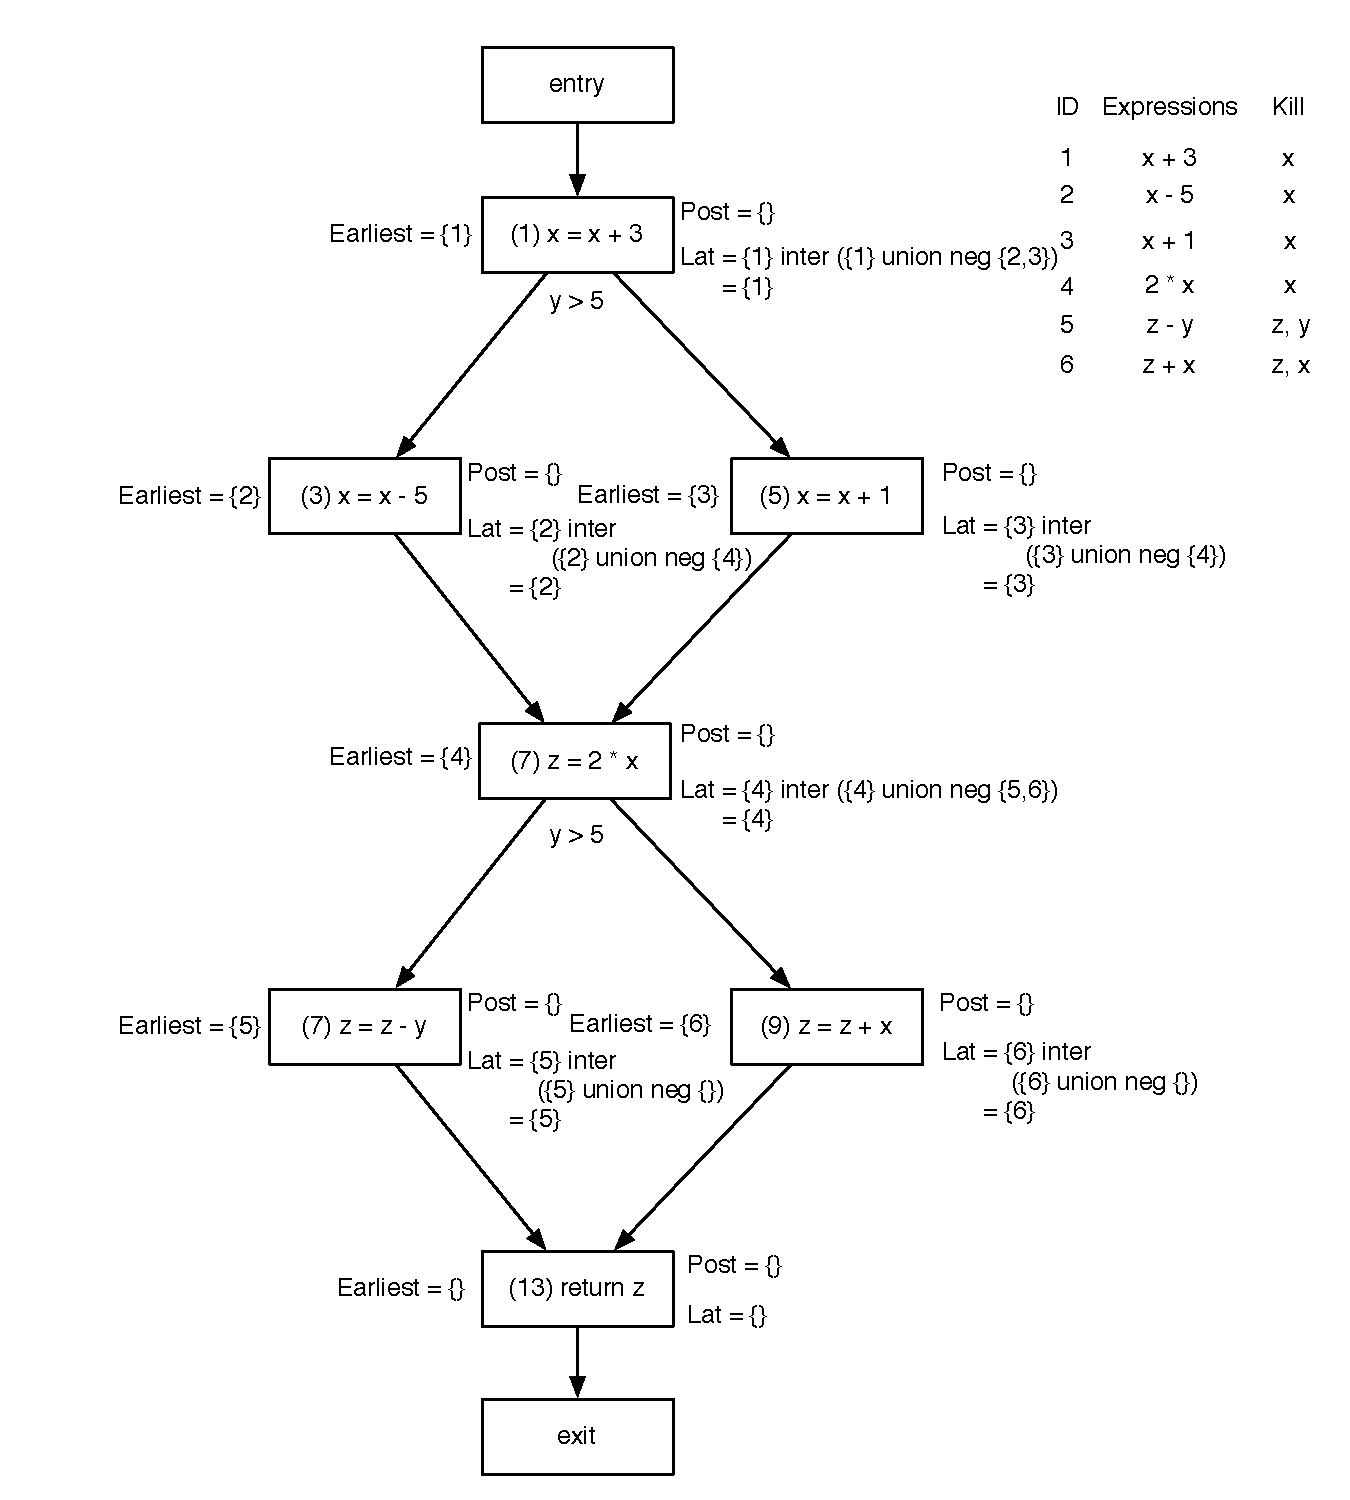
\includegraphics[scale=0.65]{cfg4_1.pdf}
    \label{fig:cfg4_1}
\end{figure}

\begin{figure}[!htbp]
    \centering
    \caption{CFG after pass 4: cleaning up.}
    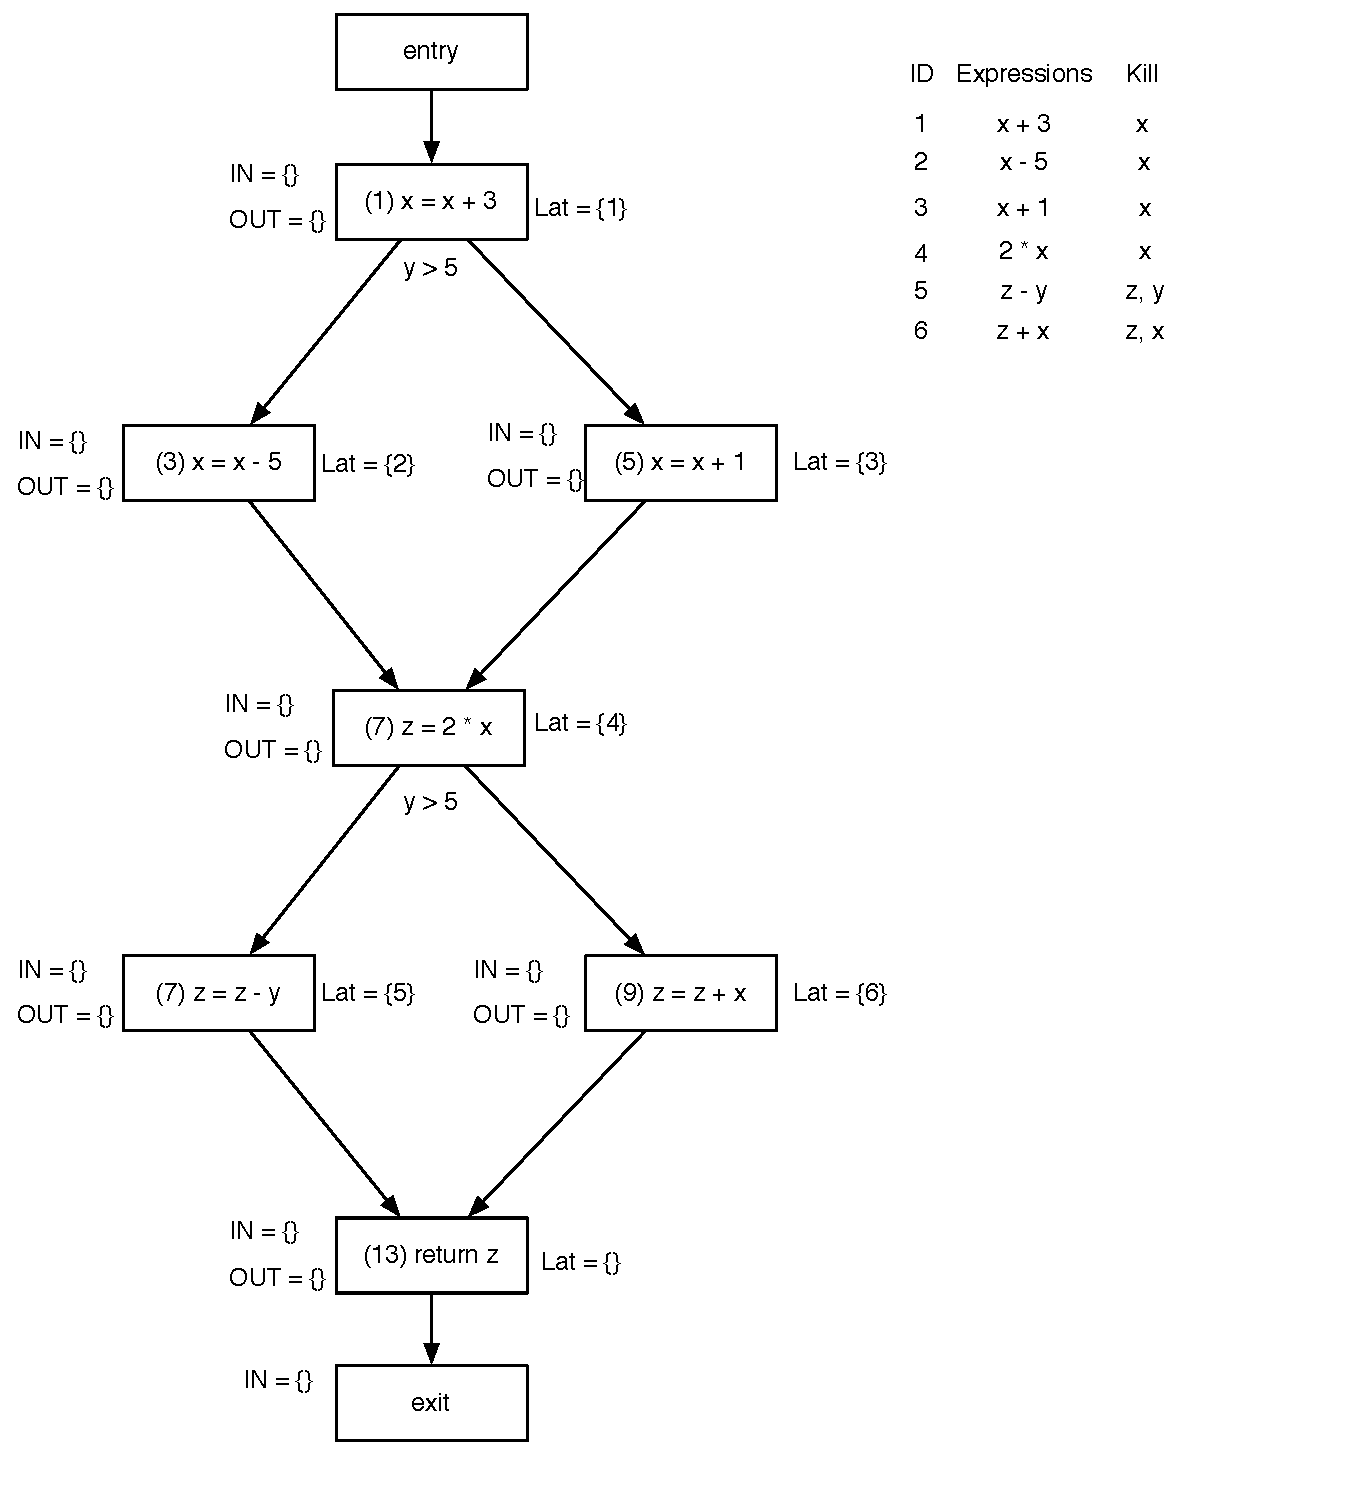
\includegraphics[scale=0.65]{cfg4_2.pdf}
    \label{fig:cfg4_2}
\end{figure}

\newpage

\subsection{LICM: Loop Invariant Code Motion}

\textbf{Loop invariant instructions:}

\begin{itemize}
   \item S2: \texttt{y = 5}
   \item S3: \texttt{q = 7}
   \item S9: \texttt{m = y + 7} (only one reaching definition: S2)
   \item S12: \texttt{r = q + 9} (only one reaching definition: S3)
\end{itemize}

S10 is not an invariant since $g$ has two reaching definitions (\texttt{g = 3} and \texttt{g = 4}).

S6 can also be considered a loop invariant, but execution can skip this block and \texttt{print} needs to print an undefined $x$ value. So if this instruction was to be moved to the pre-header, it would print $1$.

\textbf{Moved instructions by loop invariant code motion pass:}

For each statement $s$ previously listed defining $x$, we move $s$ to preheader if:

\begin{itemize}
   \item $s$ is in a block that dominates all exists of the loop,
   \item $x$ is not defined elsewhere in the loop, and
   \item $s$ is in a block that dominates all uses of $x$ in the loop.
\end{itemize}

Since S11 is dead code, we removed this instruction and moved S2 (\texttt{y = 5}) to the pre-header.

We cannot move both S9 and S12, since both may not be executed at all, which would jeopardize the program logic when the owner block is not executed.

S3 can be moved without problems because the owner block is always be executed and satisfies all the conditions we listed previously.

The final CFG is shown in Fig.~\ref{fig:loop}.


\begin{figure}[h]
    \centering
    \caption{Final loop CFG.}
    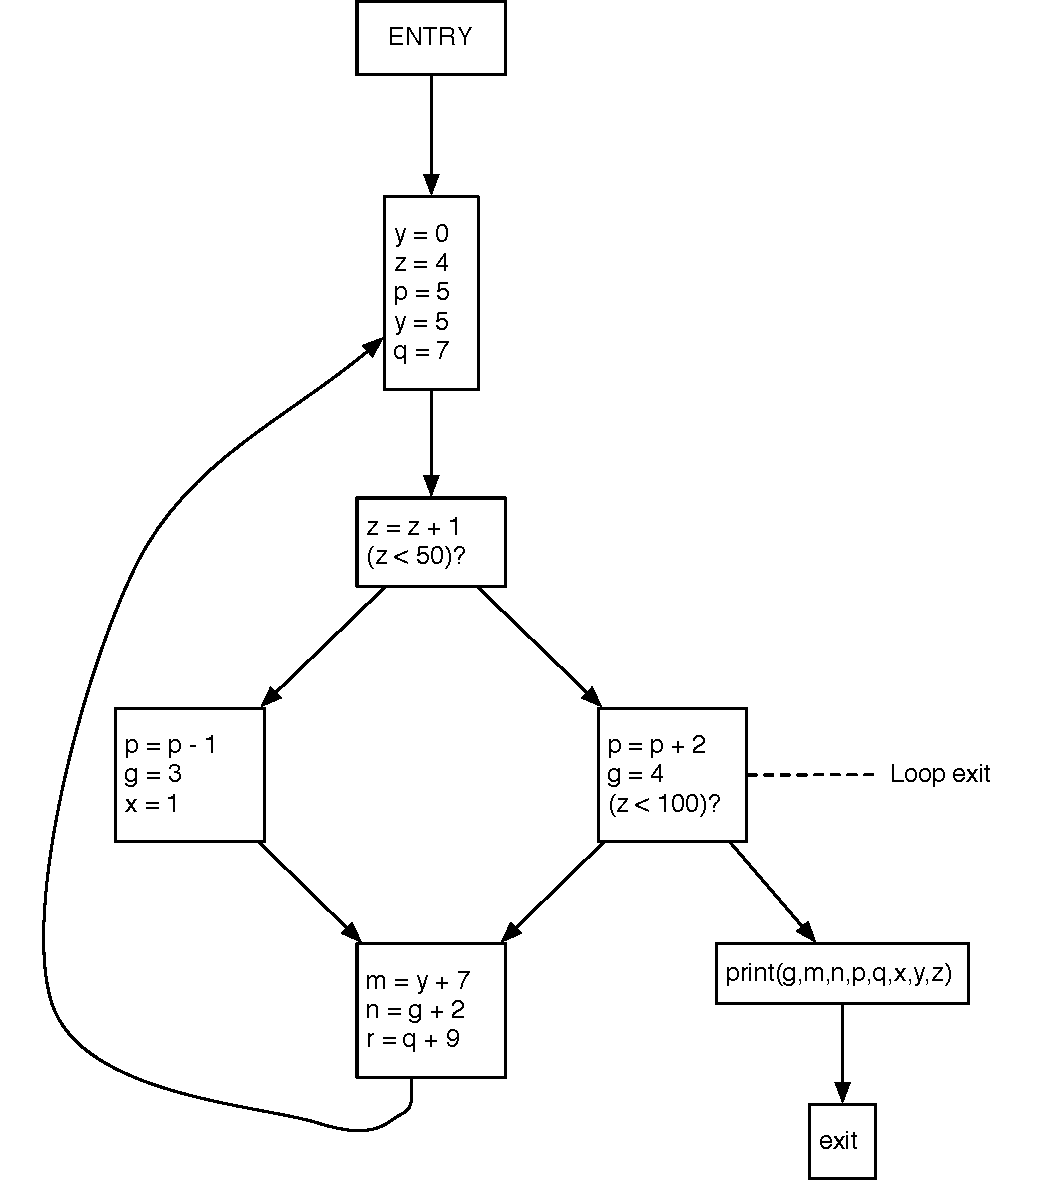
\includegraphics[scale=0.75]{loop.pdf}
    \label{fig:loop}
\end{figure}

\end{document}
